\documentclass[russian, 10pt]{beamer}

\usetheme{Madrid}
\usecolortheme{default}

\usepackage[utf8]{inputenc}
\usepackage[russian]{babel}
%\usepackage[T2A]{fontenc}

\usepackage{textcomp}
%\usepackage{a4wide}
\usepackage{bm}
\usepackage{caption}
\usepackage{subfig}
\usepackage{listings}
\usepackage{hyperref}
\usepackage{pgfplots}
\usepackage{tikz}
\usepackage{amsthm}
\usepackage{pgf,pgfarrows,pgfnodes}
\usepackage{amsmath}
\usepackage{amsfonts}
\usepackage{amssymb}
\usepackage{wrapfig}
\usepackage{indentfirst}
\usepackage{setspace}
\usepackage{graphicx}
\usepackage{textcomp}
\usepackage{array}

\usetikzlibrary{fit}
\usetikzlibrary{arrows.meta}
\usepackage{array, multirow}

\DeclareMathOperator{\E}{\mathbb{E}}
\DeclareMathOperator{\D}{\mathbb{D}}
\DeclareMathOperator{\R}{\mathbb{R}}


\usepackage{graphicx}
\usepackage[linesnumbered]{algorithm2e}

\title[Методы визуализации]
{
Задача по предсказанию, сколько потратит клиент в свой первый визит на следующей неделе
}

\author[Бобров Евгений]{Бобров Евгений}
\institute[МГУ, ВМК]{
  {\scriptsize Московский государственный университет имени М.В. Ломоносова}\\
  {\scriptsize Факультет вычислительной математики и кибернетики}\\
  {\scriptsize Кафедра математических методов прогнозирования}\\
  
}


\date{4 октября 2017}

\begin{document}

\begin{frame}
\maketitle
\end{frame}


\begin{frame}
\frametitle{Первое решение}

Первое решение состояло из двух этапов. Выделение клиентов, которые перестали посещать магазин, и разметка их нулём. Таких было около 10\% от всей выборки. Оставшиеся клиенты прогнозировались модой. Было достигнуто качество 0.37672 точности.

\begin{figure}[h!]
\begin{minipage}[h]{0.4\linewidth}
\centering
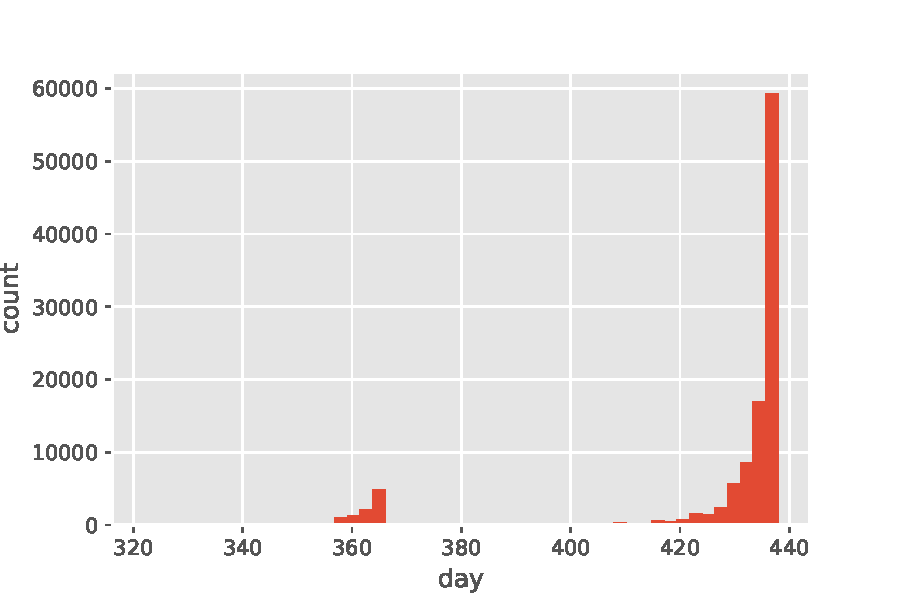
\includegraphics[scale=0.4]{images/ends.pdf}
\caption{Распределение числа последних дней в записях}
\end{minipage}
\hfill
\begin{minipage}[h]{0.5\linewidth}
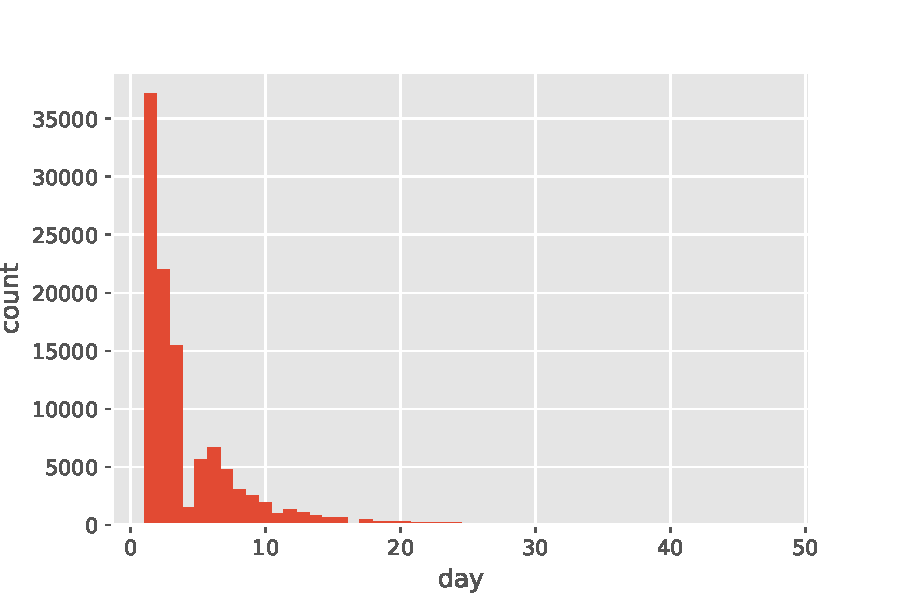
\includegraphics[scale=0.4]{images/starts.pdf}
\caption{Распределение числа первых дней в записях}
\end{minipage}
\hfill
\end{figure}

\end{frame}

\begin{frame}
\frametitle{Дальнейшие рассуждения}

Последний классы встречаются крайне редко они были слиты в один, для большей сбалансированности. Последнюю неделю я достаточно безуспешно пробовал обучать нейросети, результаты которых едва ли обходили моду. Тогда было решено обучить градиентный бустинг на стандартных признаках, что позволило с небольшим перевесом преодолеть бейзлайн на 0.39090.

\begin{figure}[h!]
\begin{minipage}[h]{0.4\linewidth}
\centering
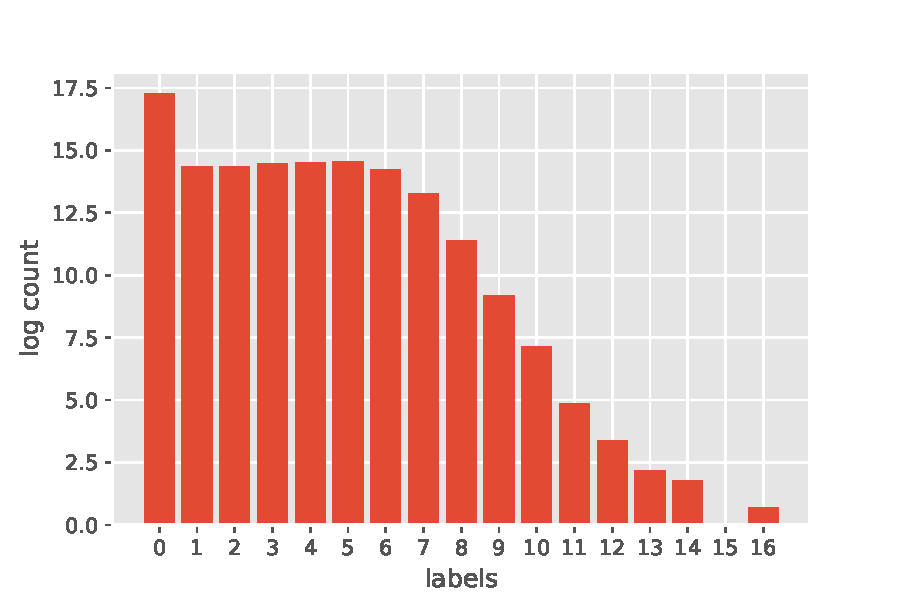
\includegraphics[scale=0.4]{images/label_distr_1.pdf}
\caption{Распределение числа меток в логарифмической шкале}
\end{minipage}
\hfill
\begin{minipage}[h]{0.5\linewidth}
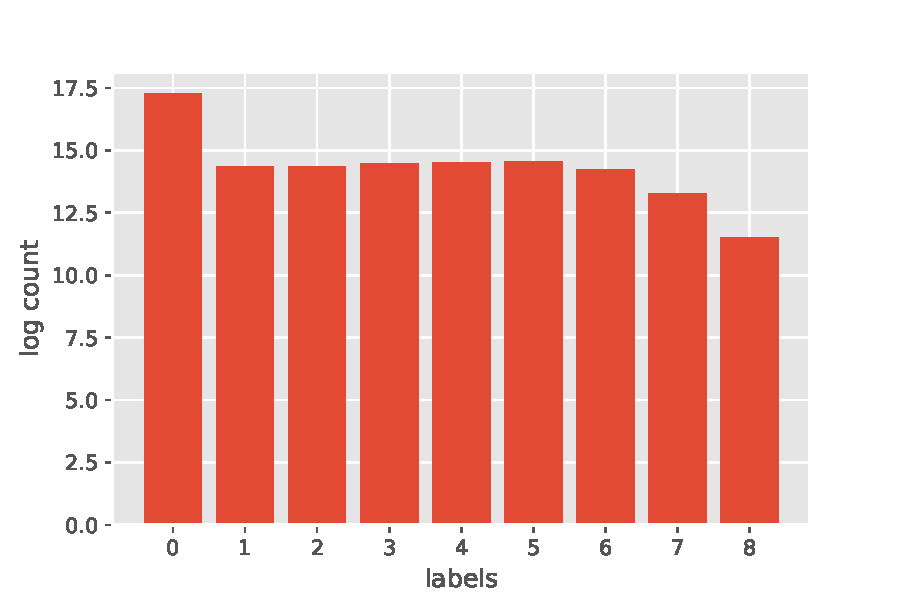
\includegraphics[scale=0.4]{images/label_distr_2.pdf}
\caption{Метки после предобработки в логарифмической шкале}
\end{minipage}
\hfill
\end{figure}


\end{frame}

\begin{frame}
\frametitle{Что за данные?}
\centering
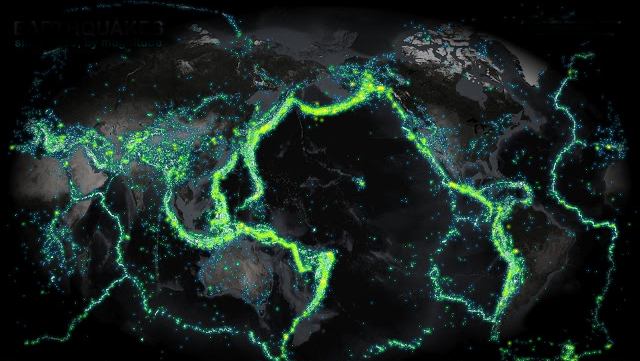
\includegraphics[scale=0.5]{images/earth.png}
\end{frame}

\end{document}